\section{ Результаты эксперимента }\label{sec:results}

Напомним условия эксперимента. Модели Ngram($n = 1$), Backoff($n = 5$) и Katz($n = 5$) запускались на тестовых выборках размером $\approx 300 MB$, что соответствует $\approx 8 \cdot 10^6$ предложений, или же $\approx \dfrac{1}{10}$ части корпуса. При этом размер алфавита был равен $|\Sigma{B^*}| = 4800$, выборки были зашумлены 3 различными способами: \KG, \BS\ и \MX. 

\subsection{ Результаты для различных моделей }

Первая часть эксперимента проводилась без оценивания уверенности ответов (см. \cref{sec:confidencemodel}) и показала следующие результаты (\cref{table:exp1}). В этой и последующих таблицах $M = Model, N = Noise, C = Confidence$.

\vspace{20pt}

\begin{table}[H]
	\begin{center}
		
		\begin{tabular}{|c|c|c|c|}\hline
			$M \backslash N$ & \KG & \BS & \MX \\ \hline
			Ngram(1) (Baseline) & 0.75 & 0.88 & 0.76 \\
			Backoff(5) & 0.89 & 0.93 & 0.90 \\
			Katz(5) & 0.961 & 0.965 & 0.962 \\ \hline 	
		\end{tabular}
		\caption{Результаты эксперимента: accuracy}
		\label{table:exp1}
	\end{center}
\end{table}

\vspace{20pt}

После того, как в первой части эксперимента хорошие результаты показала модель Katz(5), для неё были проведены испытания по поиску оптимального уровня уверенности $Confidence, C$:

\vspace{20pt}
\begin{table}[H]
	\begin{center}

\begin{multicols}{2}
	\begin{tabular}{|c|c|c|c|}\hline
		$C \backslash N$ & \KG & \BS & \MX \\ \hline
		0.9 & 0.86 & 0.94 & 0.86 \\
		0.95 & 0.979 & 0.988 & 0.981 \\
		0.97 & 0.966  & 0.986 & 0.967  \\
		0.99 & 0.94 & 0.98 & 0.95 \\ \hline 	
	\end{tabular}
\caption*{Accuracy}

	\begin{tabular}{|c|c|c|c|}\hline
		$C \backslash N$ & \KG & \BS & \MX \\ \hline
		0.9 & 0.53 & 0.43 & 0.52 \\
		0.95 & 0.61 & 0.69 & 0.62 \\
		0.97 & 0.77 & 0.85  & 0.77  \\
		0.99 & 0.91 & 0.94 & 0.91 \\ \hline 	
	\end{tabular}
\caption*{Доля классифицированных}
\end{multicols}		
\caption{Результаты эксперимента c $Confidence$}
\label{table:exp1}
\end{center}
\end{table}

\vspace{20pt}

В итоге оптимальная конфигурация -- модель Катца с $n=5$ и уверенностью $С=0.97$ ( Katz($n=5, C=0.97$) ). Она даёт высокие результаты исправления ошибок ($0.97-0.99$), классифицируя достаточно большую часть выборки ($77-85 \%$). Результаты работы этой конфигурации в будут более детально проанализированы в \cref{sec:analysis}.

Приведём также часть статистик (Precision, Recall, F-measure, Accuracy) по конкретным символам (\cref{fig:ss}):

\begin{figure}[H]
	\begin{center}
		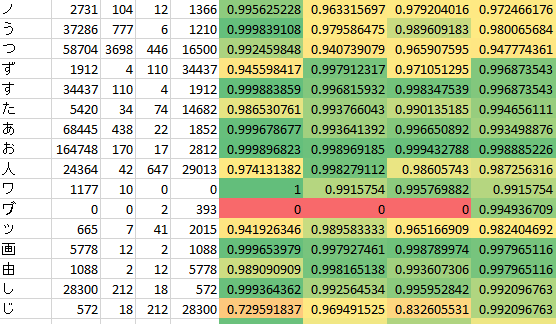
\includegraphics{table.PNG}
		\caption{Статистики по символам}
		\label{fig:ss}
	\end{center}
\end{figure}

Из полной версии этой таблицы, чо в целом хирагана исправляется чаще (0.96-0.97), чем катакана (0.93-0.95). Это можно объяснить местами их употребления: хирагана используется для подчиняющихся правилам грамматических аффиксов, а катакана -- для записи заимствованных слов, которые могут быть достаточно хаотичны. Полная версия таблицы в \cref{appendix:table}.

\subsection{ Затраты ресурсов }

Ресурсы делятся на время и память, затраты которых определяются, в нашем случае, глубиной бора $n$ и размером тестовой выборки $size$.

Ниже представлены сводные таблицы по ресурсам (\cref{table:resmem}) для различных моделей.

\begin{table}[H]
	\begin{center}
		\begin{tabular}{|c|c|c|} \hline
			Модель & Место на диске & RAM \\ \hline
			1-gram & 100 KB & $\approx$ 1 MB \\
			3-gram trie &  178 MB & $\approx$ 7 MB \\
			5-gram trie &  1.5 GB & $\approx$ 40 GB \\
			7-gram trie & 3.7 GB & $\approx$ 110 GB \\ \hline
		\end{tabular}
	\caption{Затраты ресурсов, память, $|\Sigma| = 4800$}
	\label{table:resmem}
	\end{center}
\end{table}

\begin{table}[H]
	\begin{center}
		\begin{tabular}{|c|c|c|} \hline
			Модель & 10000 примеров & 1000000 примеров \\ \hline
			1-gram & $<$ 1 мин & $\approx$ 20 мин \\
			3-gram trie &  $\approx$ 1 мин  & $\approx$ 1.5 ч \\
			5-gram trie &  $\approx$ 2 мин & $\approx$ 3 ч \\ \hline
		\end{tabular}
		\caption{Затраты ресурсов, время, $|\Sigma| = 4800$}
		\label{table:restime}
	\end{center}
\end{table}

\subsection{ Статистики по обученным моделям }

Обученные деревья даже для маленьких обучающих выборок оказываются весьма большими. Целесообразно привести статистику по 7-граммному бору (цифры для более мелких ему соответствуют, т.к. $n$-граммный бор аддитивен). См. \cref{table:trie}.

\begin{table}[H]
\begin{center}
	\begin{tabular}{|c|c|} \hline
		n	& Различных n-грамм \\  \hline
		1		&4430 \\
		2		&482607\\
		3		&3436987\\
		4		&10025503\\
		5		&19051342\\
		6		&28679559\\
		7		&37723274\\ \hline
	\end{tabular}		
\caption{Бор, $|\Sigma| = 4800$}
\label{table:trie}
\end{center}
\end{table}